\documentclass[journal]{vgtc}                % final (journal style)
%\documentclass[review,journal]{vgtc}         % review (journal style)
%\documentclass[widereview]{vgtc}             % wide-spaced review
%\documentclass[preprint,journal]{vgtc}       % preprint (journal style)

%% Uncomment one of the lines above depending on where your paper is
%% in the conference process. ``review'' and ``widereview'' are for review
%% submission, ``preprint'' is for pre-publication, and the final version
%% doesn't use a specific qualifier.

%% Please use one of the ``review'' options in combination with the
%% assigned online id (see below) ONLY if your paper uses a double blind
%% review process. Some conferences, like IEEE Vis and InfoVis, have NOT
%% in the past.

%% Please note that the use of figures other than the optional teaser is not permitted on the first page
%% of the journal version.  Figures should begin on the second page and be
%% in CMYK or Grey scale format, otherwise, colour shifting may occur
%% during the printing process.  Papers submitted with figures other than the optional teaser on the
%% first page will be refused.

%% These few lines make a distinction between latex and pdflatex calls and they
%% bring in essential packages for graphics and font handling.
%% Note that due to the \DeclareGraphicsExtensions{} call it is no longer necessary
%% to provide the the path and extension of a graphics file:
%% 
\includegraphics{diamondrule} is completely sufficient.
%%
\ifpdf%                                % if we use pdflatex
  \pdfoutput=1\relax                   % create PDFs from pdfLaTeX
  \pdfcompresslevel=9                  % PDF Compression
  \pdfoptionpdfminorversion=7          % create PDF 1.7
  \ExecuteOptions{pdftex}
  \usepackage{graphicx}                % allow us to embed graphics files
  \DeclareGraphicsExtensions{.pdf,.png,.jpg,.jpeg} % for pdflatex we expect .pdf, .png, or .jpg files
\else%                                 % else we use pure latex
  \ExecuteOptions{dvips}
  \usepackage{graphicx}                % allow us to embed graphics files
  \DeclareGraphicsExtensions{.eps}     % for pure latex we expect eps files
\fi%

%% it is recomended to use ``\autoref{sec:bla}'' instead of ``Fig.~\ref{sec:bla}''
\graphicspath{{figures/}{pictures/}{images/}{./}} % where to search for the images

\usepackage{color}
\usepackage{microtype}                 % use micro-typography (slightly more compact, better to read)
\PassOptionsToPackage{warn}{textcomp}  % to address font issues with \textrightarrow
\usepackage{textcomp}                  % use better special symbols
\usepackage{mathptmx}                  % use matching math font
\usepackage{times}                     % we use Times as the main font
\renewcommand*\ttdefault{txtt}         % a nicer typewriter font
\usepackage{cite}
%% We encourage the use of mathptmx for consistent usage of times font
%% throughout the proceedings. However, if you encounter conflicts
%% with other math-related packages, you may want to disable it.

%% In preprint mode you may define your own headline.
%\preprinttext{To appear in IEEE Transactions on Visualization and Computer Graphics.}

%% If you are submitting a paper to a conference for review with a double
%% blind reviewing process, please replace the value ``0'' below with your
%% OnlineID. Otherwise, you may safely leave it at ``0''.
\onlineid{0}

%% declare the category of your paper, only shown in review mode
\vgtccategory{Research}

%% Paper title.
\title{PeepeeEye: Interactive Exploration of Protein-Protein Interactions}

%% This is how authors are specified in the journal style

%% indicate IEEE Member or Student Member in form indicated below
\author{Katar\'{i}na Furmanov\'{a}, Kate\v{r}ina Kratochv\'{i}lov\'{a}, Jan By\v{s}ka, Ivan Viola, Eduard M. Gr\"{o}ller, Barbora Kozl\'{i}kov\'{a}}
\authorfooter{
%% insert punctuation at end of each item
\item
 Katar\'{i}na Furmanov\'{a} is with Masaryk University, Czech Republic. E-mail: furmanova@mail.muni.cz.
\item
 Kate\v{r}ina Kratochv\'{i}lov\'{a} is with Masaryk University, Czech Republic. E-mail: 374486@mail.muni.cz.
\item
 Jan By\v{s}ka is with Masaryk University, Czech Republic. E-mail: xbyska@fi.muni.cz.
\item 
Eduard M. Gr\"{o}ller is with TU Wien, Austria. Email: groeller@cg.tuwien.ac.at.
\item
Ivan Viola is with TU Wien, Austria. Email: viola@cg.tuwien.ac.at.
\item
Barbora Kozl\'{i}kov\'{a} is with Masaryk University, Czech Republic. E-mail: kozlikova@fi.muni.cz. 
}

%other entries to be set up for journal
\shortauthortitle{Furmanov\'{a} \MakeLowercase{\textit{et al.}}: PeepeeEye: Interactive Exploration of Protein-Protein Interactions}
%\shortauthortitle{Firstauthor \MakeLowercase{\textit{et al.}}: Paper Title}

%% Abstract section.
\abstract{Studying the patterns of protein interactions is fundamental for understanding the structure and function of biological complexes. The exploration of the vast space of possible mutual conformations of interacting proteins and their contact zones is very time consuming and requires non-trivial user experience. Therefore, in this paper we propose a set of novel methods for guided exploration of the conformational space which help the domain experts to select the most biochemically relevant contact zones and explore them on different levels of detail. The first method, based on customized interactive heat maps, provides the overview of all possible protein conformations and their interactive filtering. The second method enables to traverse the pre-filtered conformations using a lens view. Here the conformation in focus is equipped with the information about interacting amino acids. These techniques are interactively linked with the another proposed method which represents individual conformations in three dimensional space. The problem of high overlaps of the conformations is solved by using exploded views and open-book views. The detailed information about individual amino acids in the contact zones and their properties is presented by the last proposed technique, a list view. The usefulness of our methods was evaluated by the domain experts studying the structural maintenance of chromosomes. The results of the evaluation show that our techniques substantially decrease the time required for the exploration of all protein conformations and provide the users with information which was impossible to reveal using the existing methods.
} % end of abstract

%% Keywords that describe your work. Will show as 'Index Terms' in journal
%% please capitalize first letter and insert punctuation after last keyword
\keywords{Protein-protein interaction, heat map, exploded view, contact zone.}

%% ACM Computing Classification System (CCS). 
%% See <http://www.acm.org/class/1998/> for details.
%% The ``\CCScat'' command takes four arguments.

\CCScatlist{ % not used in journal version
 \CCScat{I.3.6}{Picture/Image Generation}%
{Line and Curve Generation};
}

%% Uncomment below to include a teaser figure.
   \teaser{
   \centering
   
\includegraphics[width=16cm]{teaser.png}
   \caption{Overview of our proposed visualization methods for the exploration of conformations of protein-protein interactions. (a) Matrix view aggregating the information about all conformations. (b) Lens view for the exploration of individual conformations and their interacting amino acids. (c) Exploded view enabling to observe the positions of individual conformations. (d) Open-book view enabling to explore the shape and constitution of the contact zones. (e) List view serving for comparison of pairing amino acids of individual conformations. TODO change image and text.}
  }

%% Uncomment below to disable the manuscript note
%\renewcommand{\manuscriptnotetxt}{}

%% Copyright space is enabled by default as required by guidelines.
%% It is disabled by the 'review' option or via the following command:
% \nocopyrightspace

\vgtcinsertpkg

%%%%%%%%%%%%%%%%%%%%%%%%%%%%%%%%%%%%%%%%%%%%%%%%%%%%%%%%%%%%%%%%
%%%%%%%%%%%%%%%%%%%%%% START OF THE PAPER %%%%%%%%%%%%%%%%%%%%%%
%%%%%%%%%%%%%%%%%%%%%%%%%%%%%%%%%%%%%%%%%%%%%%%%%%%%%%%%%%%%%%%%%

\begin{document}

%% The ``\maketitle'' command must be the first command after the
%% ``\begin{document}'' command. It prepares and prints the title block.

%% the only exception to this rule is the \firstsection command
\firstsection{Introduction}

\maketitle
Understanding the constitution and biological function of proteins is essential in many research disciplines, for example in medicine and pharmaceutics.
This knowledge is tightly connected with the ability of the protein to interact with other molecules.
Proteins can interact with small molecules, called ligands, which enter the protein.
This process, called protein-ligand docking, is widely used in protein engineering where the goal is to change specific properties of a given protein by performing a chemical reaction between the protein and a ligand.
In drug design, the protein serves as a "factory" for ligand structural changes caused again by a mutual chemical reaction. 
Such a modified ligand can then serve as a basis of a new drug. 
However, in drug design also the interactions between proteins are attracting increasing attention because most of the proteins critical for cellular life act in a cooperative manner forming multiprotein complexes. 
It is estimated that about 800 complexes exist in just one yeast cell. 
And all complexes are composed of subunits which constitute the complex via protein-protein interactions.
The main goal of the process of studying such protein-protein interactions, known as protein-protein docking, is to identify an appropriate spatial \textbf{conformation} of interacting proteins.
The conformation is represented by the mutual spatial orientation of the interacting proteins.
Each conformation contains a \textbf{contact zone} consisting of the set of amino acids from both interacting proteins which are in the interaction distance spanning from 3 to 5 \AA ngstr\"{o}ms.
In other words, the contact zone is positioned on the interface between the proteins and is formed by mutually interacting amino acids.

Structure determination of protein-protein interactions in laboratories is very challenging as well as time and money consuming.
This is due to many problems related to the dynamic nature of the proteins, the difficulties with their purification and the preparation of samples.
Therefore, computational docking helping with an early understanding of the feasibility of proposed conformations between interacting proteins is currently a very promising option.
Many algorithms and tools appeared in this respect in the last years.
A categorization of the existing algorithms along with the description of their basic principles was published recently by Huang~\cite{Huang2014}.
However, these tools are producing a large number of possible conformations.
The domain expert has to explore them and select the most biochemically relevant ones. 
Therefore, the next step is to enhance the exploration process by other computational tools with visual support.
There were already several algorithms published for re-ranking of the conformations according to different criteria thus suggesting the user those conformations which should be explored in detail.
As a representative of these attempts, Malhotra et al.~\cite{Malhotra2015} in 2015 presented DockScore, a webserver for ranking the individual conformations produced by the docking tools. 
Their idea is based on building a scoring scheme considering several interface parameters, such as surface area, hydrophobicity, spatial clustering, etc.
This helps the user to reduce the number of conformations to a smaller set which still has to be explored manually.
For this exploration the visual support is essential, enabling to see the spatial orientation of the contact zones and hot spot amino acids and to compare different conformations.
Figure~\ref{fig:dockscore} shows the visual representation of two different conformations which combines traditionally used techniques, i.e., cartoon and balls\&sticks rendering.
The green and yellow proteins represent two different docking solutions with respect to the violet protein. 
The amino acids in red and blue illustrate an individual hot spot of the two corresponding contact zones.

\begin{figure}[bt]
  \centering
  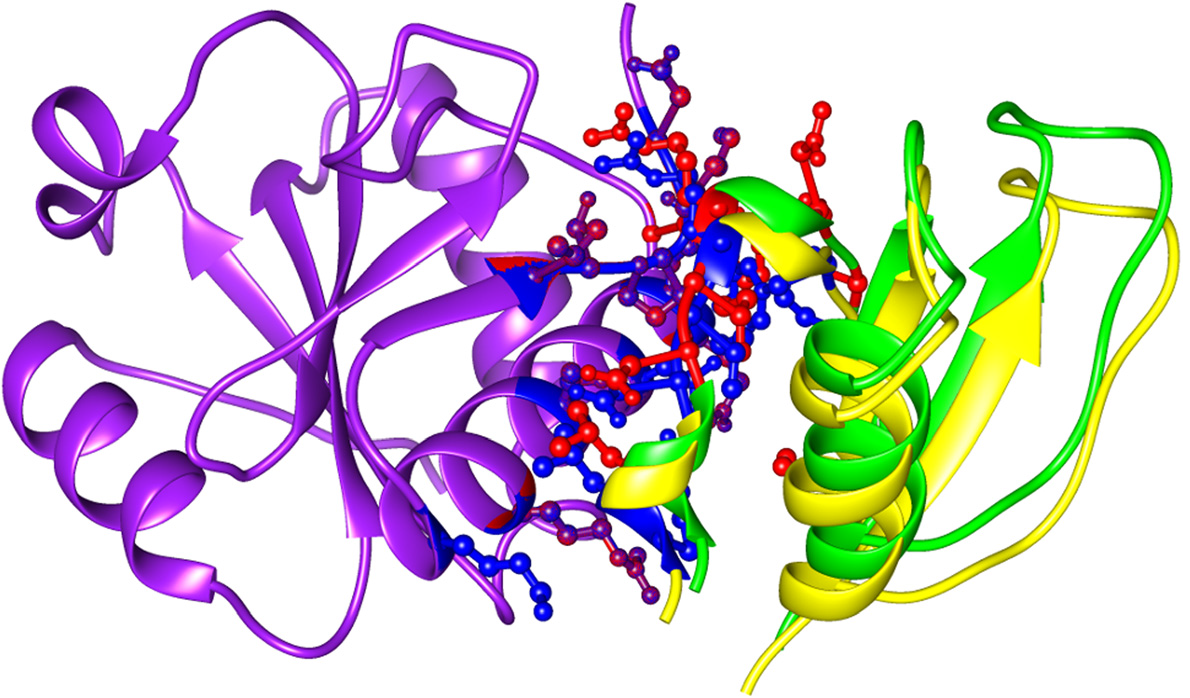
\includegraphics[width=0.8\columnwidth]{dockscore.png}
  \caption{Visual representation of the native and computed conformations of the protein complex with PDB ID 1SYX. Image taken from~\cite{Malhotra2015}.}
  \label{fig:dockscore}
\end{figure}

It is clearly visible that even for the comparison of two conformations the traditional representation suffers from many occlusion problems and it is hard to perceive the differences between individual solutions.
When comparing more conformations, even without a detailed visualization of hot spot amino acids, the problem becomes even more apparent (see Figure~\ref{fig:problem}).

\begin{figure}[tb]
  \centering
  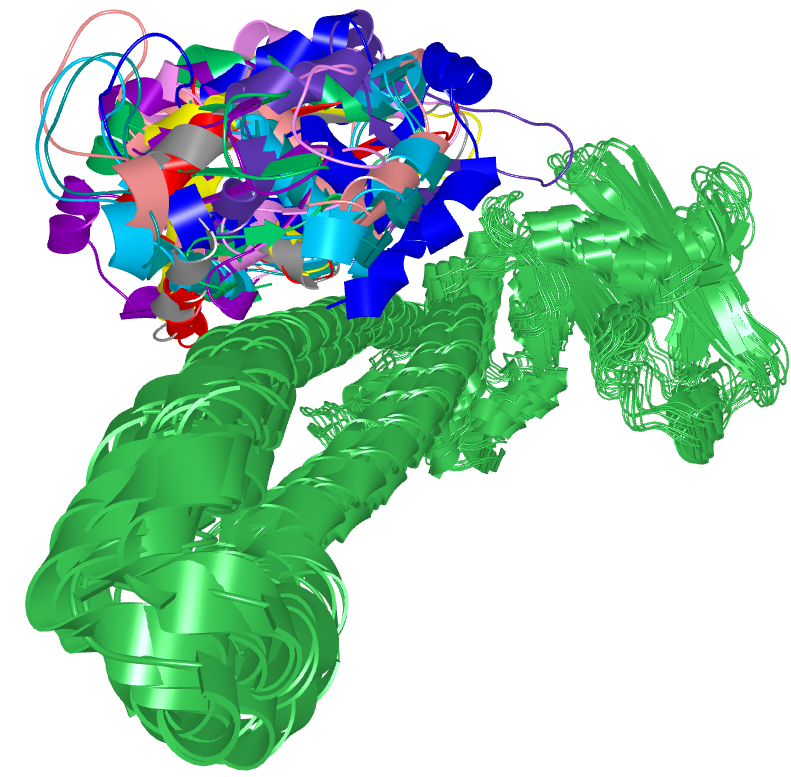
\includegraphics[width=0.7\columnwidth]{problem.png}
  \caption{Superimposition of several possible conformations between two proteins visualized using traditional cartoon rendering. The set of green protein instances corresponds to one of
the interacting proteins, the colored components represent the second protein in different conformations.}
  \label{fig:problem}
\end{figure}

Therefore, in this paper we are proposing a solution to this clutter problem.
We present a set of novel methods for the visualization and comparison of individual conformations.
They aim to remove the problems of existing solutions and provide the domain experts with an intuitive and user friendly tool for an interactive exploration of protein-protein interactions provided by the computational tools.
Our solution is designed for dealing with a large number of conformations so the user is not forced to apply any of the re-ranking algorithms before using our solution. 


\section{Related Work}
In this section we review the existing techniques related to our proposed representations of protein-protein interactions.
Generally, molecular visualization represents very important and useful topic in visualization.
This was confirmed also by Kozlikova et al.~\cite{Kozlikova2015} in their survey of molecular visualization techniques.

The issue of visual representation of protein-protein interactions can be tackled from different perspectives.
One group of existing solutions focuses on the visualization of entire networks of interacting proteins.
Because of their complexity, i.e., the number of interacting proteins, the visualizations are mostly graph-based.
Jeanquartier et al.~\cite{Jeanquartier2015} presented a survey of databases enabling the visual analysis of protein networks.

The second group consists of techniques visualizing the contact zones and their interacting amino acids.
The spatial techniques have to deal with the problem of occlusion and visual clutter caused by the fact that the most interesting parts of the interacting proteins, the contact zones, are positioned close to each other (see Figure~\ref{fig:varshney}a).
In other words, without any transformation or a visual enhancement (e.g., through transparency) it is impossible to visually explore the contact zones.
Therefore, Jin et al.~\cite{Jin2014} presented the open-book view where the interacting proteins are rotated to orient the contact zones towards the camera.
The problem of the presented solution lies mainly in the missing information about the interacting amino acids and the unified coloring of the contact zones.
An alternative approach presented by Lee and Varshney~\cite{Varshney2003} computes and visualizes the intermolecular negative volume and the area of the docking site (Figure~\ref{fig:varshney}b,c).
This way the users can observe the volume between the interacting proteins without direct visualization of the contact zones themselves.
This can serve the domain experts as an interactive tool for studying possible docking conformations.

\begin{figure}[bt]
  \centering
  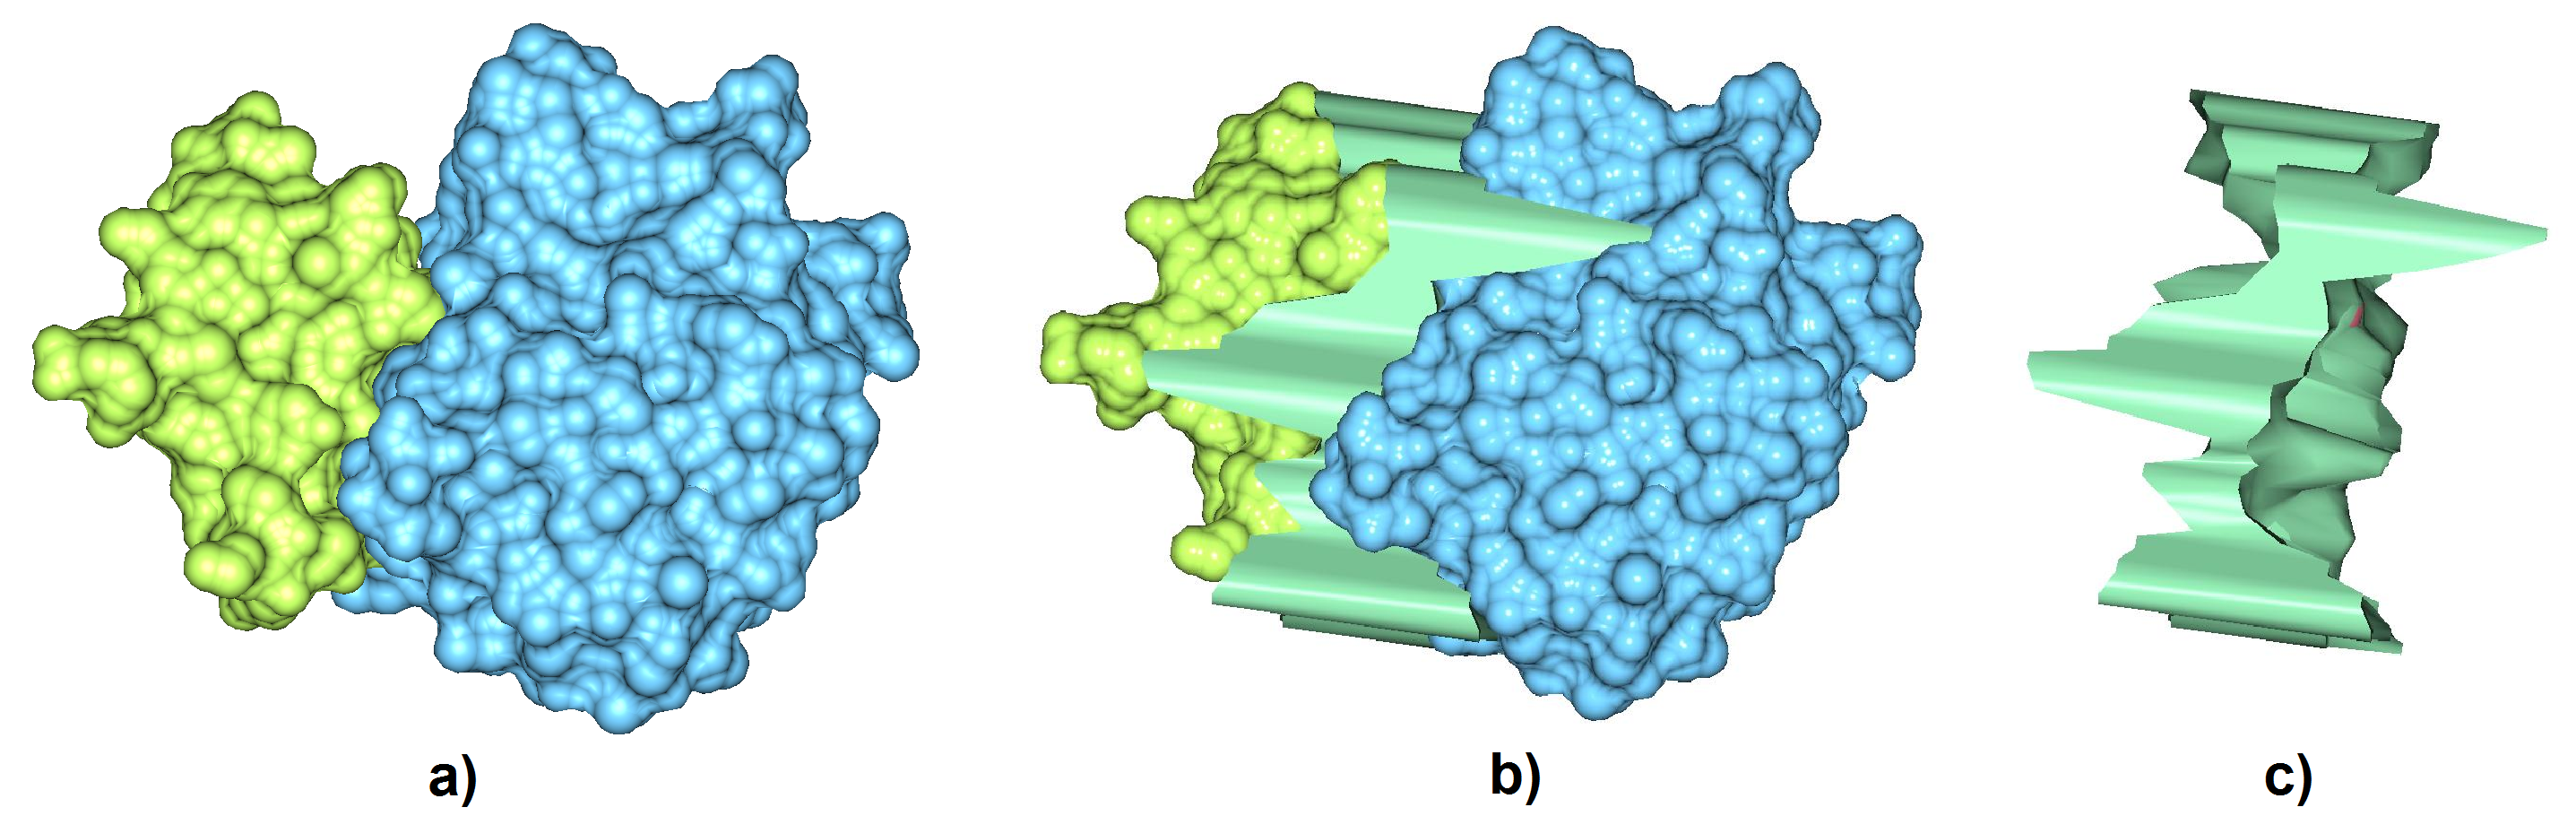
\includegraphics[width=1.0\columnwidth]{varshney.png}
  \caption{(a) Surface visualization of two interacting proteins with PDB ID 4SGB where the contact zones are not visible. (b) and (c) Visualization of the intermolecular negative surface representing the volume between the contact zones. Image taken from~\cite{Varshney2003}.}
  \label{fig:varshney}
\end{figure}

One of our proposed spatial visualizations adopts the idea of so called exploded views.
This technique enables to observe the parts of objects which are originally hidden.
Bruckner et al.~\cite{Bruckner2006} adopted this technique to volume data and demonstrated it on the scans of different parts of human body.

Alternative approaches to the visualization of contact zones may use abstracted 2D representations.
As an example of such an approach the schematic representation of the contact zones used in the PDBsum database~\cite{pdbsum} can be taken (see Figure~\ref{fig:pdbsum}). 
In an overview visualization each of the interacting proteins is represented by a sphere equipped with the information about the number of amino acids forming the contact zones and the number of different types of interactions between them (e.g., salt bridges, disulphide bonds, hydrogen bonds, or non-bonded contacts).
Another detailed visualization lists all contact-zone amino acids. 
The interactions are visualized by lines of different colors and thicknesses which represent the type and strength of the interaction.

\begin{figure}[bt]
  \centering
  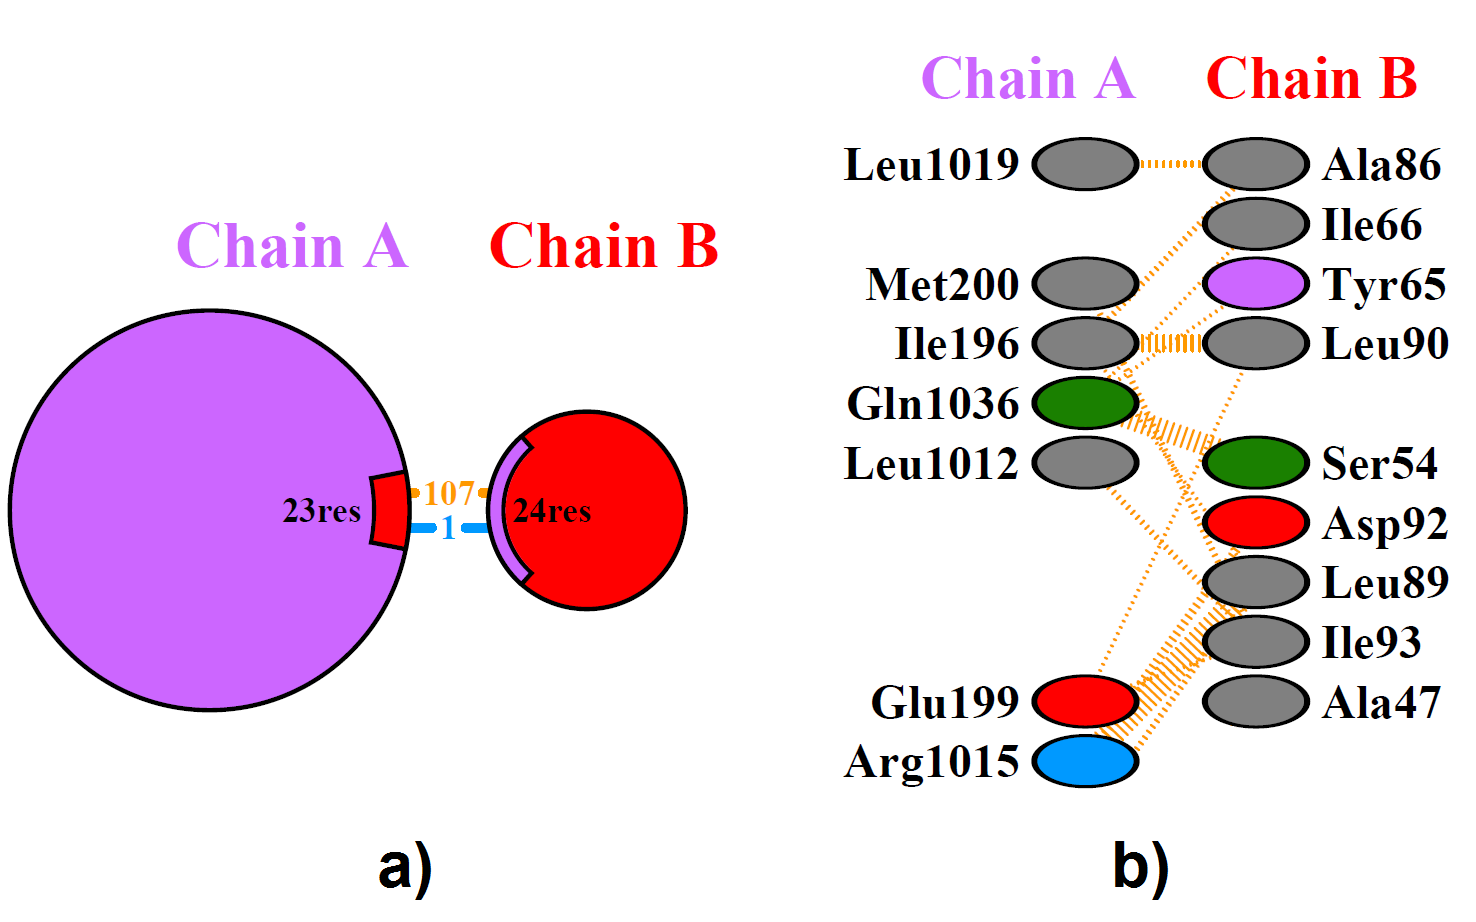
\includegraphics[width=1.0\columnwidth]{pdbsum.png}
  \caption{Two abstracted visualizations of the complex SMC3-Scc1 with PDB ID 4UX3 available in the PDBsum database. (a) Overview representation showing the number of amino acids in the contact zones and the types on interactions. (b) Part of the list of all interacting amino acids along with individual interactions and their strength. Images taken from the PDBsum database~\cite{pdbsum}.}
  \label{fig:pdbsum}
\end{figure}

Abstracted representations were already successfully applied to protein-ligand docking.
Byska et al.~\cite{Byska2015} proposed visual abstractions of tunnels serving for ligand transportation and their evolution in molecular dynamics simulations.
Their ATH and STH representations show heat maps encoding the information about tunnel openness over time.
The MoleCollar visualization shows the evolution of the shape of the narrowest part of the tunnel, its bottleneck.
The visualization contains also the information about the position and a set of physico-chemical properties of amino acids surrounding the tunnel bottleneck.

Lex et al.~\cite{Lex2012} proposed the visual analysis tool serving for exploration of large-scale heterogeneous genomics data for characterization of cancer subtypes.
They use different views onto the complex data and one of them is the method for comparison of different datasets.
The abstracted representation shows the similarities in the datasets by connecting the corresponding blocks of data. 
The thickness of the connections denotes the amount of similarities.
This representation is to some extent similar to our proposed InCo lens view but in our case it focuses more on the exploration of the interacting amino acids in individual conformations.

In another proposed method, the Conformation Matrix View, we tackle the problem of visualizing many items in a limited 2D space.
It often leads to very small space available for individual items which are then hard to perceive.
Therefore, we also had to adopt one of the interactive lens techniques which were thoroughly surveyed by Tominski et al.~\cite{Tominski2014}.


\section{Overview}
Our newly proposed visualizations aim to help the domain experts to explore a set of possible conformations detected by one of the existing computational tools and to select the most biochemically relevant ones.
The relevance consists of both geometrical fitting of the contact zones and the chemical compatibility between interacting amino acids which is derived from their physico-chemical properties.
Therefore, the users have to iteratively filter out those conformations which are not fulfilling specific given criteria.
To follow this workflow, summarized in Figure~\ref{fig:workflow}, we propose a set of specific visualizations. 
The input datasets consisting of dozens of conformations between two interacting proteins were computed using HADDOCK~\cite{haddock}, one of the currently most often used tools.
In the following sections we describe our newly proposed techniques which visually support and enhance the exploration workflow.

\begin{figure}[bt]
  \centering
  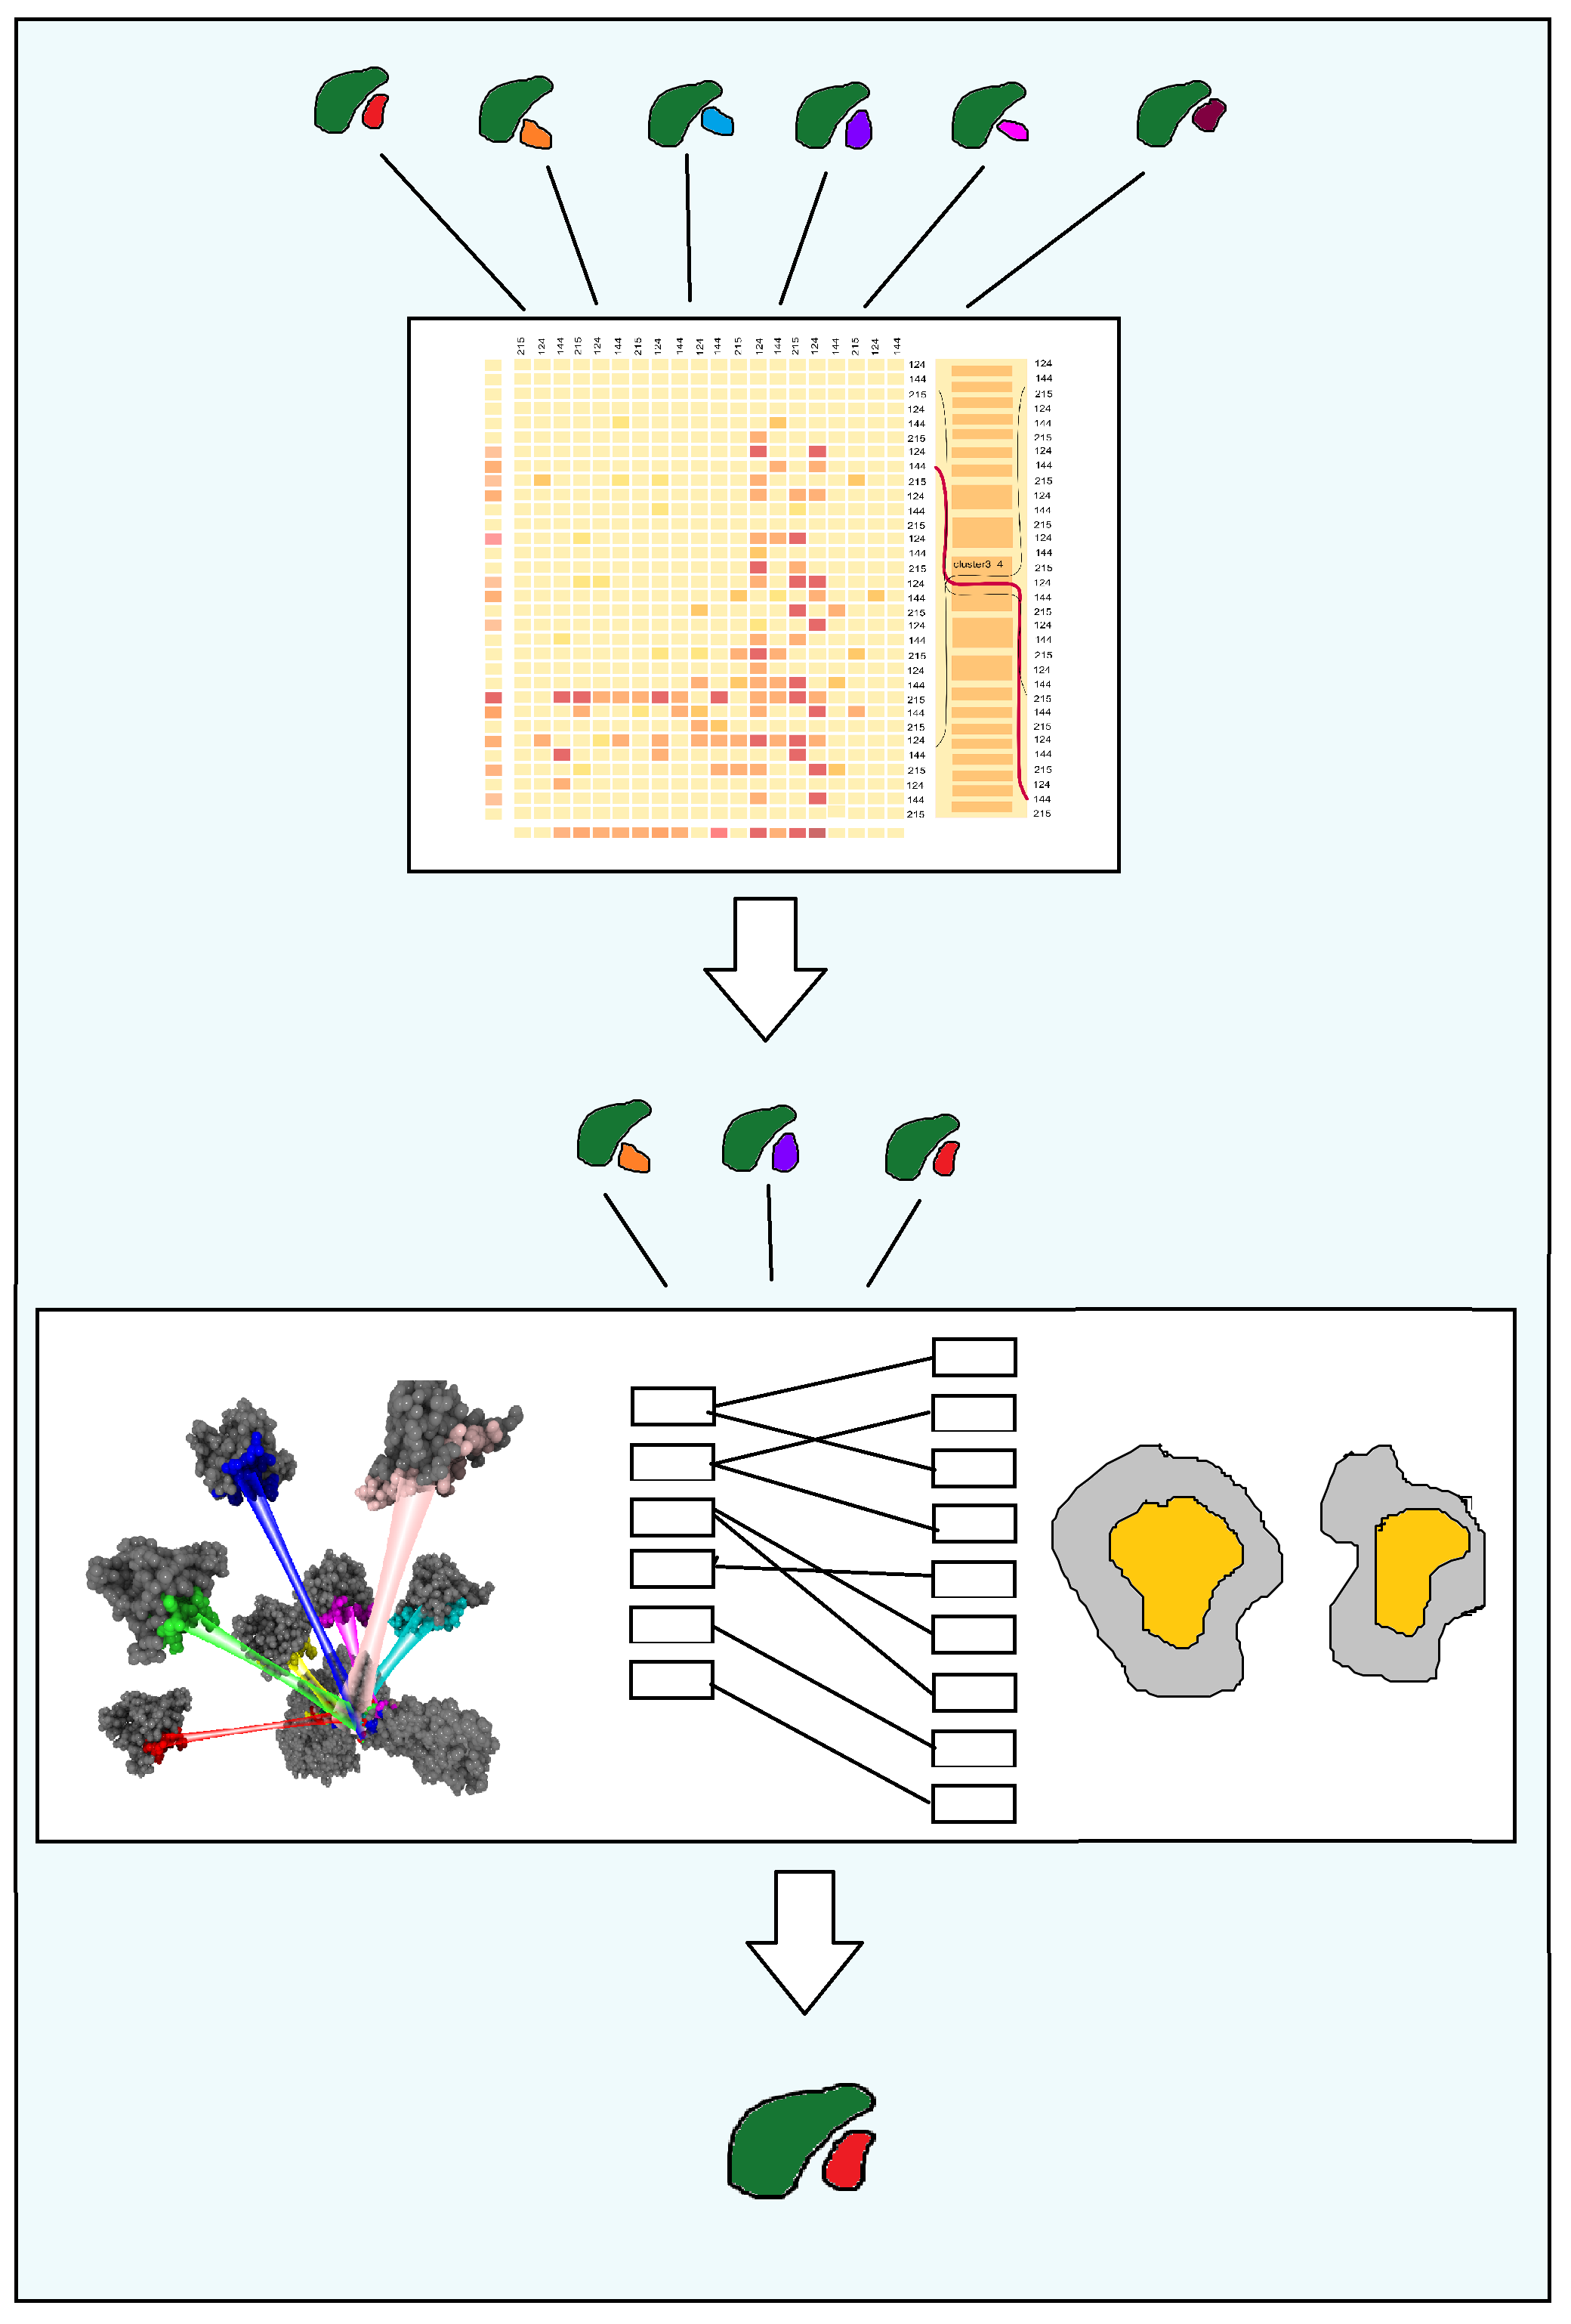
\includegraphics[width=1.0\columnwidth]{workflow.png}
  \caption{Overview of the process of exploration of the input conformations using our newly proposed methods.}
  \label{fig:workflow}
\end{figure}

\section{CMV -- Conformation Matrix View}
If the biochemists have some preliminary knowledge about the interacting proteins and know about a pair of amino acids from these proteins that they are surely interacting, they can give this information as an input parameter directly to the computational tool.
If no such information is available, the tool searches for possible conformations randomly.
In both cases, the resulting set of conformations is large and requires some preliminary filtering.
This filtering can be based on the prior knowledge or can consider those pairs of amino acids which are present in most of the resulting conformations.
To support this task, we propose a matrix-based visualization inspired by commonly used heat maps (see Figure~\ref{fig:matrixlens} left part).
The rows and columns of the conformation matrix view (CMV) correspond to two interacting proteins.
Each row or column represents one amino acid present in a contact zone of some of the conformations. 
In other words, the rows and columns are formed only by those amino acids of the interacting proteins which are in contact in at least one conformation.
The contact between the amino acids is based on their Euclidean distance. 
Two amino acids are considered to be in contact if their distance is between 3 and 5 \AA ngstr\"{o}ms.
The color of each rectangle in the matrix corresponds to the number of the occurrences of the corresponding interacting amino acids in the set of conformations. 
The intense red color represents pairs of amino acids which are interacting in most of the conformations.
Thus, it can be anticipated that they play a significant role in the protein-protein interaction and it is meaningful to explore them in more detail.
On the other hand, rare combinations of amino acids can be filtered out.
The matrix serves directly for filtering out those improbable solutions by interactive selection of rectangles (cells of the CMV).
Moreover, the matrix allows the selection of a combination of more pairs of amino acids.
This is useful if the user wants to further explore only those conformations which contain the interactions between amino acids $A$, $B$ and/or simultaneously also $C$, $D$. 

\begin{figure}[bt]
  \centering
  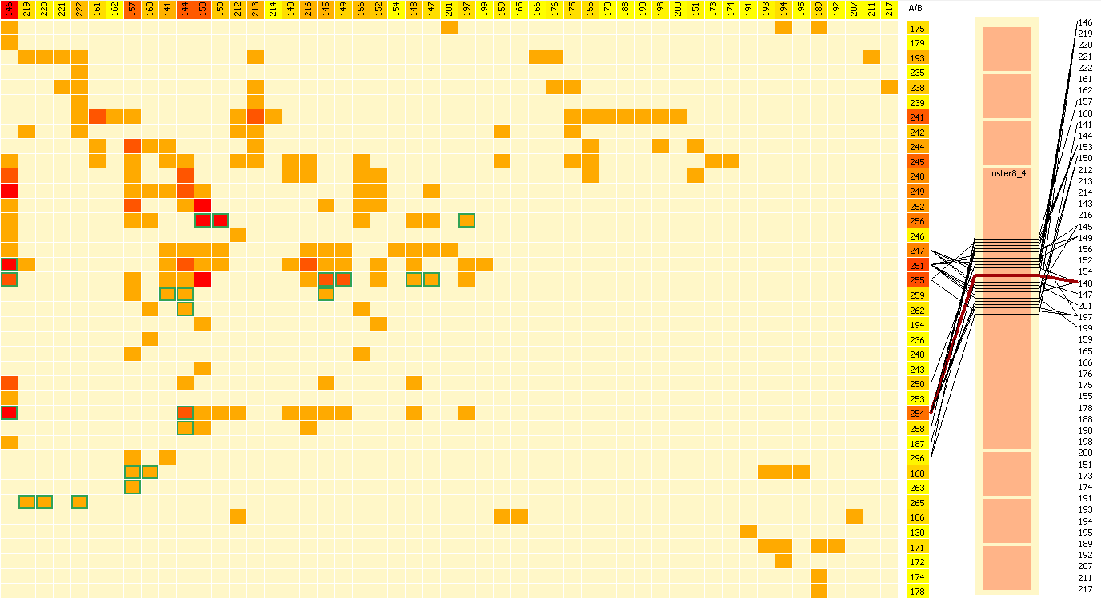
\includegraphics[width=1.0\columnwidth]{matrixlens.png}
  \caption{Matrix view (left) showing the aggregated information about the presence of mutually interacting amino acids in all conformations. It is interactively linked with the lens view (right) presenting more detailed information about individual conformations and their interacting amino acids. \textcolor{red}{TODO change image}}
  \label{fig:matrixlens}
\end{figure}

The rows and columns in the matrix can be also sorted according to the frequency of occurrence of the amino acids in the conformations. 
This results in the concentration of more frequent pairs of amino acids in the top left corner of the matrix (see Figure~\ref{fig:sort}).

\begin{figure}[bt]
  \centering
  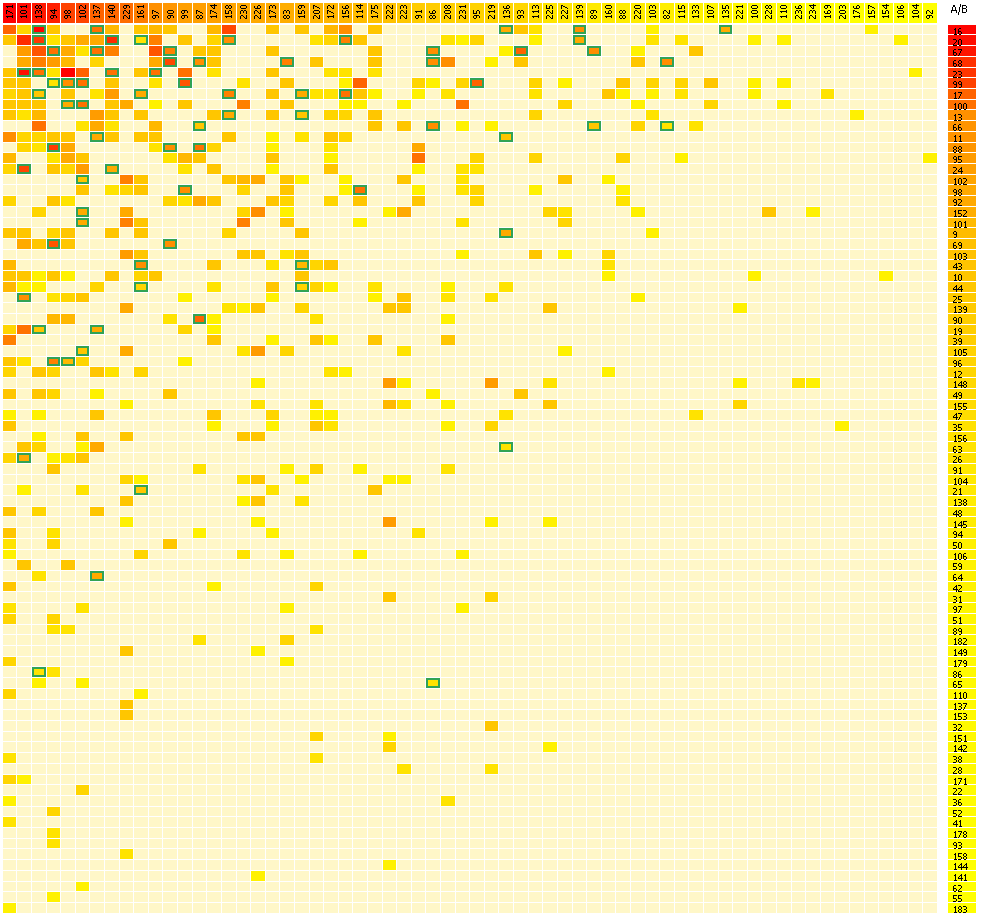
\includegraphics[width=0.8\columnwidth]{sort.png}
  \caption{Matrix view sorted according to the frequency of occurrence of the amino acids in all conformations. Green borders of some rectangles represent the pairs which are present in some of the conformations (selected in the lens view).}
  \label{fig:sort}
\end{figure}

One of the biggest advantages of the matrix view is its independence on the size of the input set.
The number of rows and columns is limited by the size of interacting proteins, so in the worst case it can correspond to the total number of amino acids of these proteins.
However, usually the number of amino acids in the contact zones is very limited -- for medium-size proteins there can be approximately from 10 to 20 amino acids.
So the number of rows and columns is much smaller than this upper limit.
Then, each conformation of the input dataset increases the counters represented by the color in the matrix rectangles.
Therefore, the only parameter influencing the size of the matrix is the size of the interacting proteins.
For large proteins the rectangles of the matrix can be too small.
In such situations, the users can use the table lens technique introduced by Rao and Card~\cite{Rao1994} applied to both rows and columns of the matrix.

The matrix view is interactively linked with another newly proposed visualization, lens view, positioned directly next to the matrix (Figure~\ref{fig:matrixlens} right part). 

\section{InCo Lens View}
InCo lens accompanying the matrix view provides the users with more detailed information about individual conformations.
In the matrix view the information about all conformations is merged in order to give an overview of the interacting amino acids concerning the entire dataset.
Therefore, the constitution of individual conformations, yet very important in the filtering stage, is omitted.
Our lens view complements the conformation matrix view and presents the content of the contact zones of individual conformations in a highly abstracted way.

\textcolor{red}{TODO IMAGE!!!}

The central part of the lens view consists of rectangles representing individual conformations. 
The biggest rectangle in focus (in the center) corresponds to the currently investigated conformation. 
It contains the identifier of the conformation and the connection between the closest amino acids in the corresponding contact zones (highlighted by the polyline).
The lens view is highly interactive and closely linked with the matrix view.
The user can hover the mouse over the lists of amino acids on the left and right side and the corresponding connection lines for a given amino acid are appearing.
By clicking on the rectangle representing the amino acid the connection lines remain in the view.
The user can scroll the view with the mouse wheel and explore individual conformations.
The pairs of amino acids forming the conformation in focus can be highlighted in the matrix view (green borders of rectangles in Figure~\ref{fig:sort}) so the user can immediately see the number of conformations in which these pairs are present as well.
Vice versa, by interacting with the matrix view and selecting given rectangles, the lens view can be automatically filtered and shows only those conformations which satisfy the filtering condition defined in the matrix view.

By combining the matrix and lens views, the domain expert can inspect the large input set of conformations and primarily assess their biochemical relevance.
Selected conformations can be further processed by the following visualization methods.

\section{CEV -- Conformation Exploded View}
The biochemists are already well accustomed with the manipulation of molecules in a three-dimensional environment, thus this space has to be an integral part of the workflow.
However, as already stated, exploring and comparing many structures in 3D at once suffers from problems with high overlaps, occlusion, and visual clutter. 
So the traditionally used representations are not sufficient (as indicated in Figures~\ref{fig:dockscore} and~\ref{fig:problem}).
To overcome these limitations, we use the technique of so called exploded views which enlarges the distance between the interacting proteins (see Figure~\ref{fig:exploded}). 

\begin{figure}[bt]
  \centering
  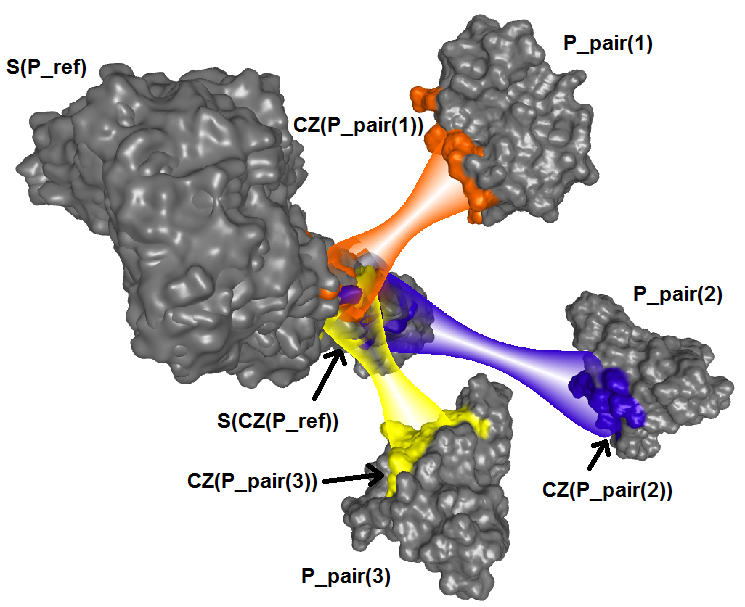
\includegraphics[width=1.0\columnwidth]{exploded.png}
  \caption{Exploded view showing the interaction between the reference protein and its paired proteins. Proteins are represented by their surface and the contact zones are colored.}
  \label{fig:exploded}
\end{figure}

The main principle is the following.
First the user selects one of the interacting proteins as the reference one.
Lets mark the second protein in this interaction as the paired protein.
All these reference proteins taken from the selected conformations are aligned using a Combinatorial Extensions structural alignment algorithm~\cite{Shindyalov1998} (see the green protein in Figure~\ref{fig:problem}).
The set of proteins interacting with the reference proteins are positioned around these reference proteins.
As it is expected that the set of conformations selected in the previous stage contains more items, the paired proteins are overlapping significantly.
Therefore, by increasing the distance between the reference and paired proteins using exploded views can remove this issue.
To ensure that the paired proteins in the exploded view will not collide with each other, we have to calculate their spatial position based on their bounding boxes.
To maintain the information about the position of the contact zones on both reference and paired protein, we display their connection as a tube surrounding the connection between the centers of the contact zones.
The radius of the tube at each point of the segment is modulated by its distance to the segment endpoints.
The opacity of the tube is modulated in screen space, depending on the distance to the segment centerline.

The resulting visualization removed not only the problem of overlapping paired proteins but also enabled the user to see the contact zones which were in the original position of interacting proteins hidden between them (see Figures~\ref{fig:case2} and~\ref{fig:case3}).
However, this solution does not solve the problem that the contact zones are still facing each other so the user has to manipulate with the camera to observe the contact zone from a perpendicular view. 
But even such manipulation does not enable to see both contact zones at once (the second contact zone is then located on the opposite side of the camera).
This problem is solved by the open-book view presented in the following section.

\section{Open-Book View}
This view is activated when the user selects one of the conformations from the exploded view. 
Then the visualization of other conformations is suppressed and the open-book view is launched.
This view consists of the animation in which the reference and paired proteins are rotated and translated so that they are positioned next to each other and their contact zones are facing towards the observer (see Figure~\ref{fig:book}). 
To maintain the information about the pairing of amino acids, the user can visualize also individual connections by simple lines.

\begin{figure}[bt]
  \centering
  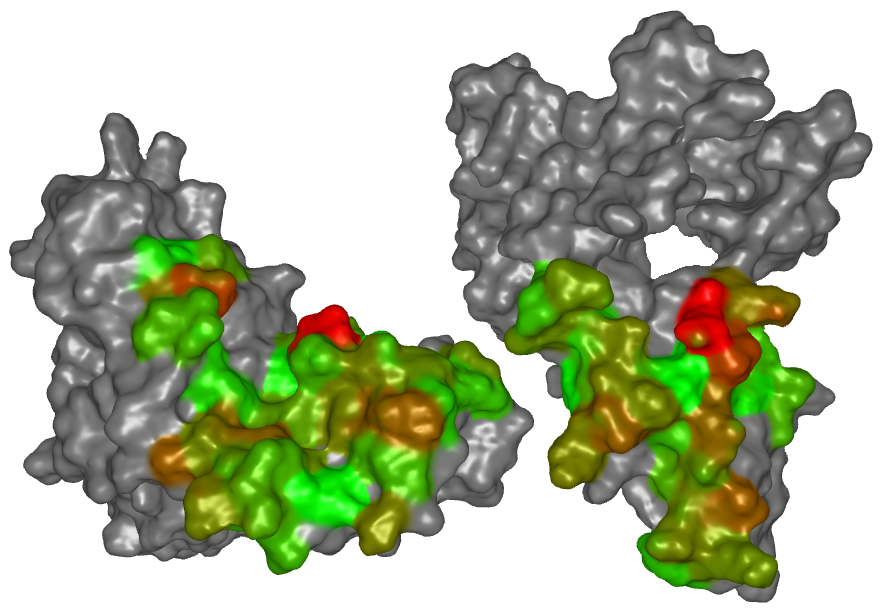
\includegraphics[width=0.8\columnwidth]{book.png}
  \caption{Open-book view enabling to explore the contact zones between the interacting proteins simultaneously. The surface of the contact zones can be color-coded according to different criteria -- here the color represents the distance between the pairs of amino acids. \textcolor{red}{TODO change image, programming still in progress}}
  \label{fig:book}
\end{figure}

The contact zones represented by their surface can be color-coded according to different criteria.
The color can correspond the mutual distance between the amino acids -- the closest amino acids have different color than the most distant ones.
It can also represent different physico-chemical properties of the amino acids or their atoms, such as hydrophobicity or partial charges.
To inform the users about the types and identifiers of individual amino acids, the surfaces can be equipped with labels bearing this information.

In both the exploded view and the open-book view the protein can be represented also by other traditionally used visualization methods, such as cartoon, spheres, balls\&sticks, sticks, etc.
Moreover, these methods can be combined so, for example, the proteins can be represented by cartoon method and the amino acids in the contact zones can be visualized using sticks representation to see their spatial orientation (see Figure~\ref{fig:contact}).

The combination of exploded view and open-book view is very useful for exploration of individual conformations.
But when the task is to compare individual conformations with respect to the pairs of interacting amino acids, these views can give only a limited information.
Therefore, we proposed another abstracted view serving mainly for the comparison of the paired amino acids in individual solutions.

\section{List View}
The list view consists of two sets of amino acids in the contact zones, each set coming from one interacting protein (see Figure~\ref{fig:list}).
The left part contains all amino acids coming by default from the reference protein, the right part is formed by their counterparts in the paired protein.
However, the order of proteins in the list view can be changed.
The view contains all possible connections (wrt. the mutual distance) between amino acids from both contact zones.
To avoid cross sections of lines representing the connections, some amino acids on the right side can be repeated -- one occurrence for each amino acid in the reference protein in the maximal distance of 5 \AA. 
The user can also select between two modes -- the compact list view and the compare list view.
The difference lies in the positioning of the amino acids in the left part of the list view. 
In the compare mode, each amino acid has its fixed position and when this amino acids is not present in the contact zone for some conformation, its position is filled with white rectangle with the name of the missing amino acid (see Figure~\ref{fig:list} right).
The compact mode ignores the missing amino acids and arranges the amino acids to the most compact form to save space (Figure~\ref{fig:list} left).
 
For each conformation one list view is created and all list views are juxtapositioned so the user can see and visually compare the constitution of the contact zones of all selected conformations.
The user can interact with this representation by changing the properties of the amino acids mapped onto their corresponding rectangles (same properties as those mapped onto the surface in the 3D views) and sort the left part of the list according to them (see Figure~\ref{fig:sorting}).
Moreover, by clicking on individual rectangles representing amino acids, the corresponding amino acids are selected in the 3D view as well.

\begin{figure}[bt]
  \centering
  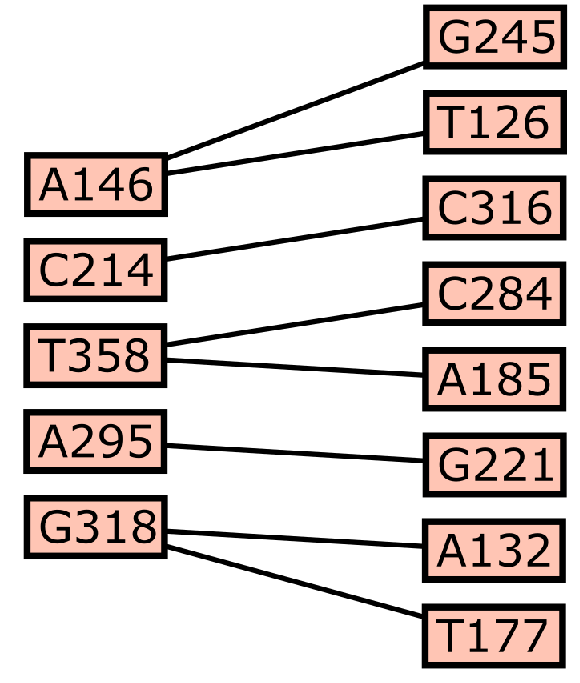
\includegraphics[width=1.0\columnwidth]{list.png}
  \caption{Compact list view (left) showing all pairs of amino acids from interacting proteins which are in the interaction distance. Compare list view (right) serves better for comparison of different conformations. It preserves the blank space for amino acids which are in the contact zone in some of the conformations but not in this particular one. \textcolor{red}{TODO change image}}
  \label{fig:list}
\end{figure}

\begin{figure}[bt]
  \centering
  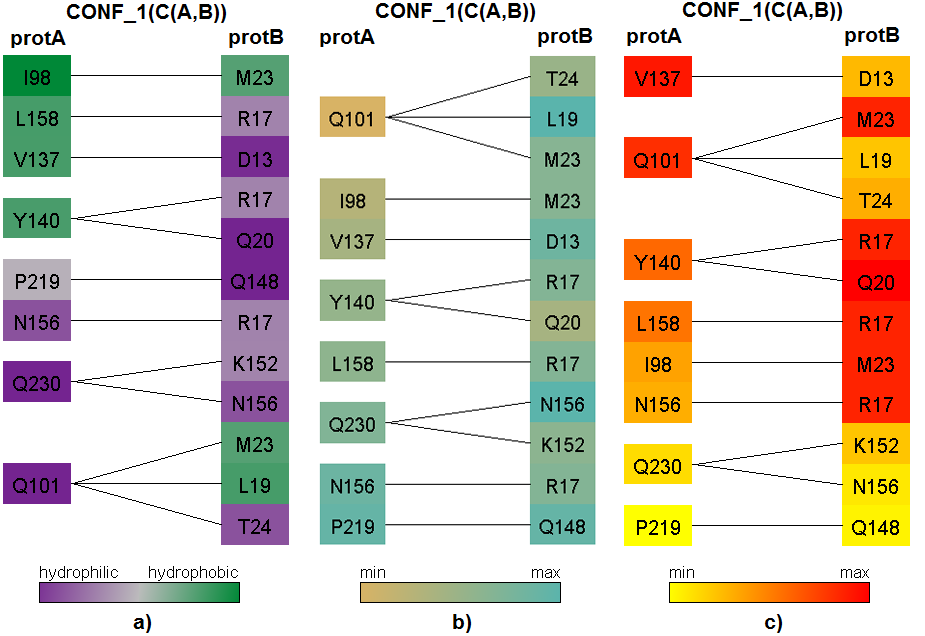
\includegraphics[width=1.0\columnwidth]{sorting.png}
  \caption{Sorting of the list view according to different properties of amino acids -- hydrophobicity (left), mutual distance (middle), frequency of occurrence (right). \textcolor{red}{TODO change image, add legend to the image}}
  \label{fig:sorting}
\end{figure}


\section{User Interaction}
Except for the interaction with individual visualizations which were described along with their principles, all proposed visualizations are interactively linked to support the workflow of the biochemists as much as possible.
It means that by the selection of rectangles in the matrix view the user automatically filters out those conformations which do not fulfill the filtering criteria and these conformations are further omitted from the exploded, open-book, and list views as well.
Of course, the user can anytime return to the beginning of the process and by iterative refining of the filtering using the matrix and lens views the set of conformations can be further narrowed.
Another possible scenario is that the user reveals that some of the promising conformations was filtered out at the beginning.
Such conformations can be then returned back to the exploration process.

\section{Demonstration and Results}
All presented techniques were designed in tight cooperation with the domain experts from the field of functional genomics and proteomics.
Their current main research focus is on structure maintenance of chromosome (SMC) complexes~\cite{Hudson2011,Guerineau2012,Palecek2015}. 
The SMC complexes are key players in chromatin organization where they ensure the proper condensation of chromosomes. 
The researchers analyze the architecture and function of such complexes using a variety of experimental approaches. 
Their goal is to uncover the way the subunits of these complexes interact with each other and execute unique function(s) of these complexes. 
Therefore, a visual representation of such information is highly beneficial because it helps to reveal the spatial relationships between the subunits in an intuitive way.

To demonstrate the usability of our proposed techniques, the domain experts selected an example of the hNSE1-hNSE3 complex.
The crystal structure of this complex present in human genome was already examined in detail and the resulting conformation is already published in the PDBsum database under the PDB identifier 3NW0. 
\textcolor{red}{TODO this info will be shaped by Honza Palecek on Tuesday}
Therefore, it can serve as a testing complex for both computational tools as well as our proposed visualizations.
In this case the domain experts provided the computational tools with the prior knowledge about one pair of interacting amino acids, Leucine with ID 97 from the reference protein and Methionine with ID 23 from the paired protein.
They selected the web version of the HADDOCK tool for producing the set of possible conformations. 
The tool resulted in 40 conformations grouped into 10 clusters (each containing 4 conformations).
The conformations belonging to one cluster are considered to be very similar according to internal HADDOCK score and evaluation.

These 40 conformations were loaded to our proposed matrix and lens views. 
The matrix immediately shows one very interesting result.
Even when the user sets the input pair of amino acids, only a small portion of the resulting conformations really contains this interaction.
In our particular case, only in five conformations (all conformations from cluster 1 and one conformation from cluster 5) the Leucine 97 and Methionine 23 amino acids were in the interacting distance (less than 5 \AA ).

Our conducted user study is divided into two parts. In the first part we suppose that we have the knowledge about the interacting pair of amino acids stated above.
The second case will be more complicated because we will not take this information into account and will evaluate the conformations without any prior knowledge.

\subsection{Case Study 1 -- Guided}
In this case when we had already the information about two interacting amino acids, the matrix view enables to select the suitable conformations immediately.
However, when no such information is known, the matrix serves as a preliminary filter which can be further smoothed by using the lens view.
The interacting pairs of amino acids can be preliminary explored using this view thus help the biochemist to further filter out the irrelevant conformations.

In the next step, the selected conformations (five of them in our case) are passed to the next stage where they are explored in 3D view.
Here one of the proteins is selected as the reference one and all conformations are structurally aligned with respect to this reference protein.
The paired proteins are positioned around the reference ones.
Figure~\ref{fig:case1} shows the situation when the five conformations are visualized using the traditional method.
Conformations are represented as a surface and the contact zones are highlighted using different colors.
However, the most interesting parts, the contact zones, are completely hidden.

\begin{figure}[bt]
  \centering
  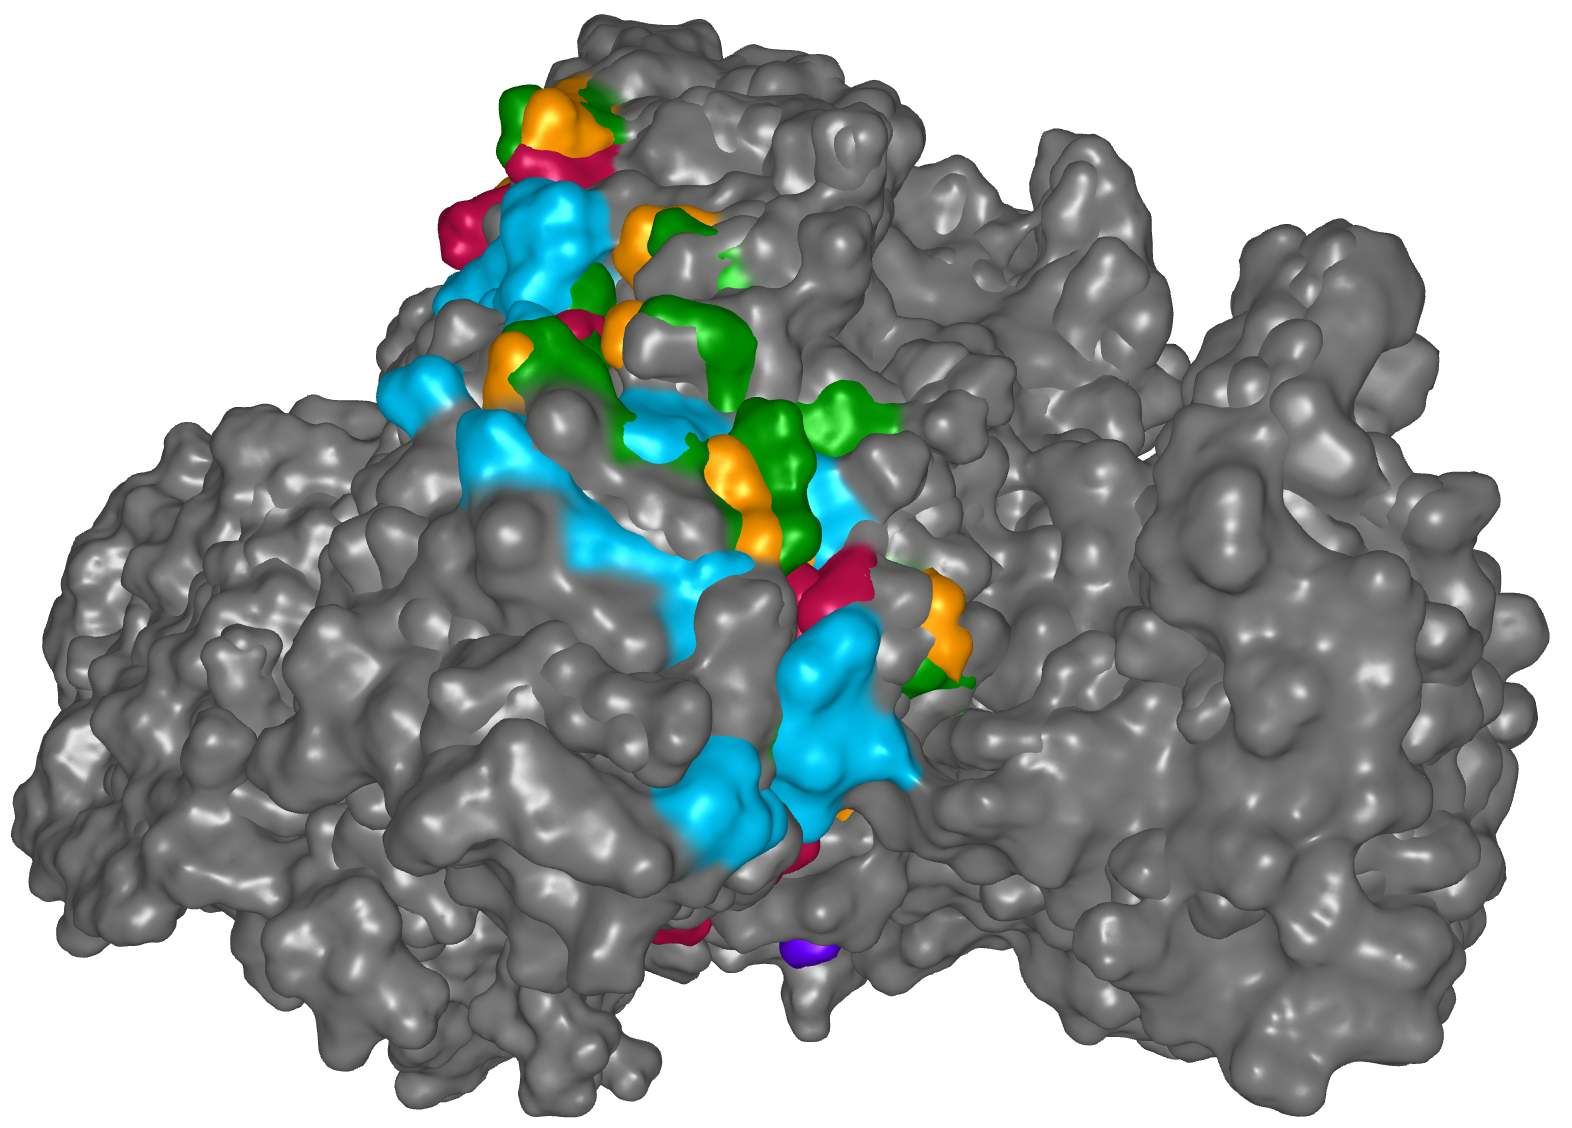
\includegraphics[width=0.7\columnwidth]{case1.png}
  \caption{Five conformations represented by surfaces with highlighted contact zones. It is clearly visible that such a representation is insufficient for observation and comparison of the contact zones.}
  \label{fig:case1}
\end{figure}

Our exploded view overcomes this limitation (Figure~\ref{fig:case2}) and shows all paired proteins in an appropriate distance from the reference protein so all proteins are not overlapping.
The individual contact zones on the paired proteins are now clearly visible and the user can also see the differences between the positions of the contact zones in the reference protein.

\begin{figure}[bt]
  \centering
  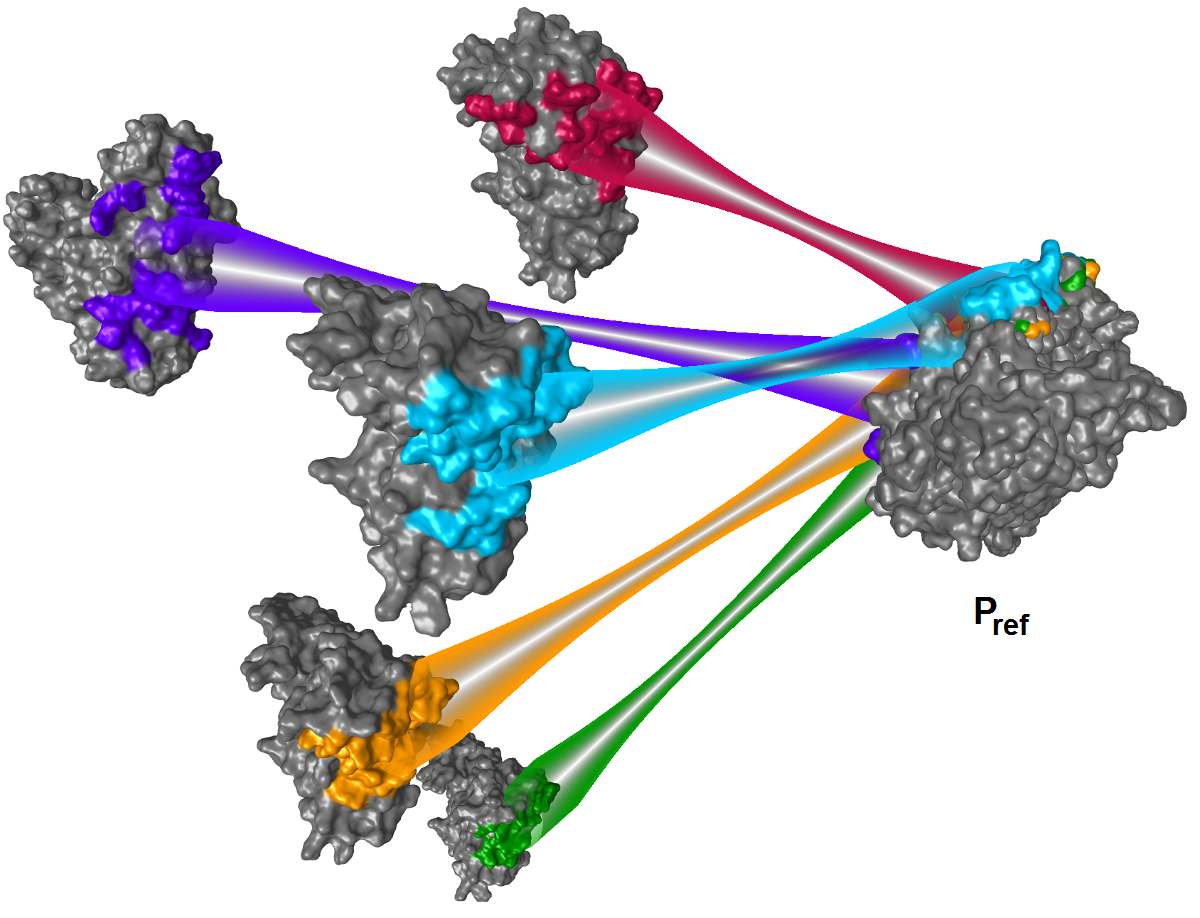
\includegraphics[width=1.0\columnwidth]{case2.png}
  \caption{Five conformations represented by the exploded view.}
  \label{fig:case2}
\end{figure}

The user can further explore the constitution of the contact zones in detail by using the open-book view where the individual amino acids can be highlighted using a different visualization method. 
Figure~\ref{fig:contact} shows the combination of cartoon representation (green part belongs to the contact zone) with balls\&sticks representation of Leucine 97 and Methionine 23 colored according to their hydrophobicity.

\begin{figure}[bt]
  \centering
  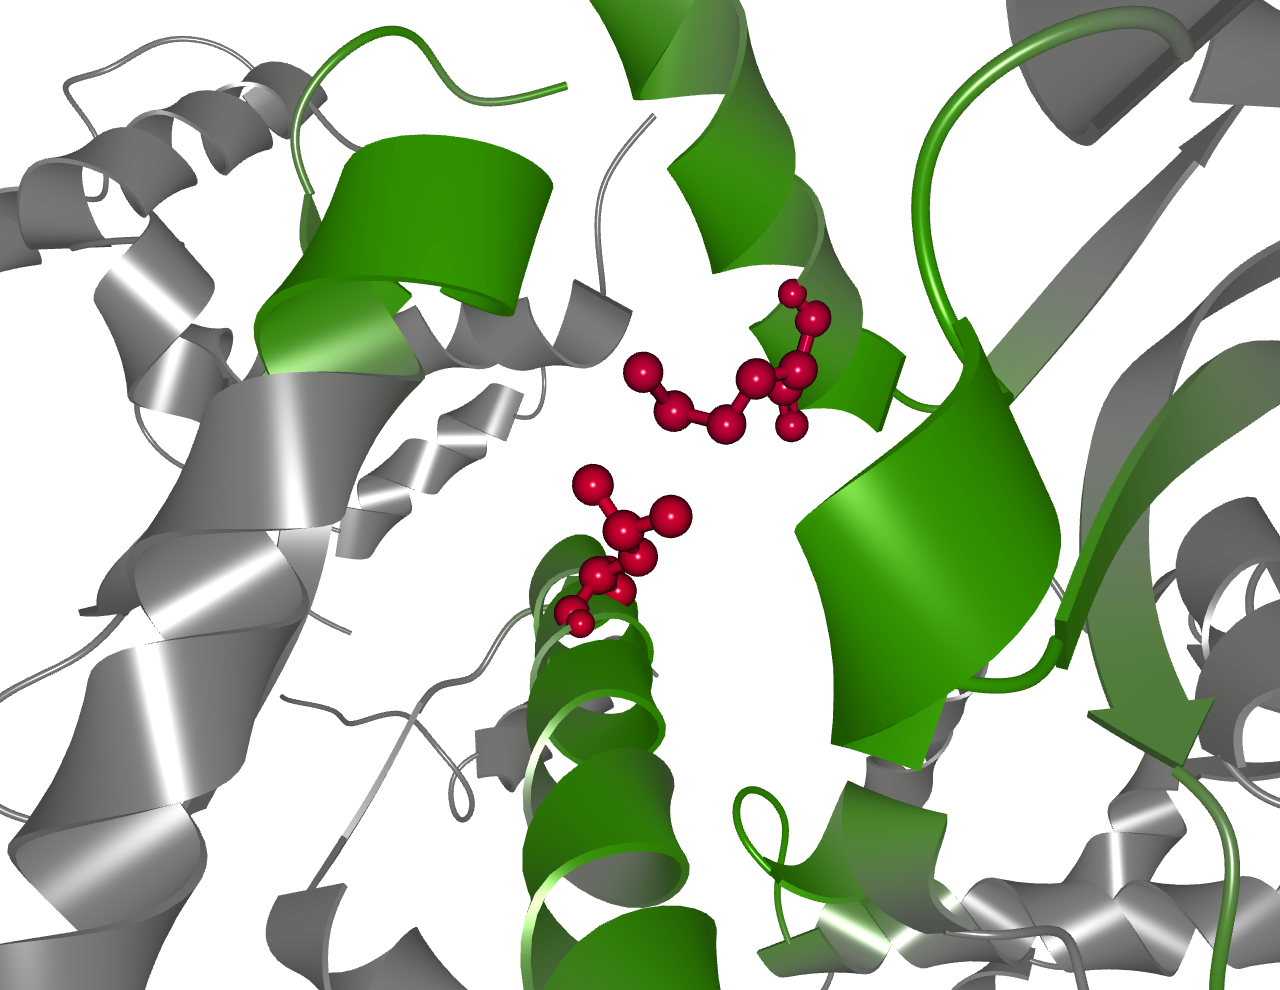
\includegraphics[width=0.8\columnwidth]{contact.png}
  \caption{Cartoon representation of the interacting proteins where green color corresponds to the contact zone. Leucine 97 and Methionine 23 interacting amino acids are highlighted using the balls\&sticks method and the color corresponds to their hydrophobicity. \textcolor{red}{TODO change image}}
  \label{fig:contact}
\end{figure}

The five conformations can be also compared using the list view.
This view gives clear information about changes in the contact zones.
Figure~\ref{fig:case3} shows the resulting list views for our five conformations.
The left part of the views contains the list of amino acids in the contact zone of the reference protein, right part represents the paired protein.
From this view it is clearly visible that the contact zone of the conformation named as $cluster5_4$ contains much less amino acids in the reference protein than the other conformations.
On the other hand, conformations $cluster1_1$, and $cluster1_3$ are the most similar with respect to the number and type of amino acids. 
The conformations can be then compared pairwise as well and the list view immediately reveals the differences in their sets of amino acids.

By different sorting applied to the reference protein on the left side the user can observe the hydrophobicity, mutual distance, or occurrence in all scrutinized conformations.
The reference and paired proteins can be switched so the paired protein will be positioned in the left side and the sorting can be performed on it as well.

\begin{figure*}[bt]
  \centering
  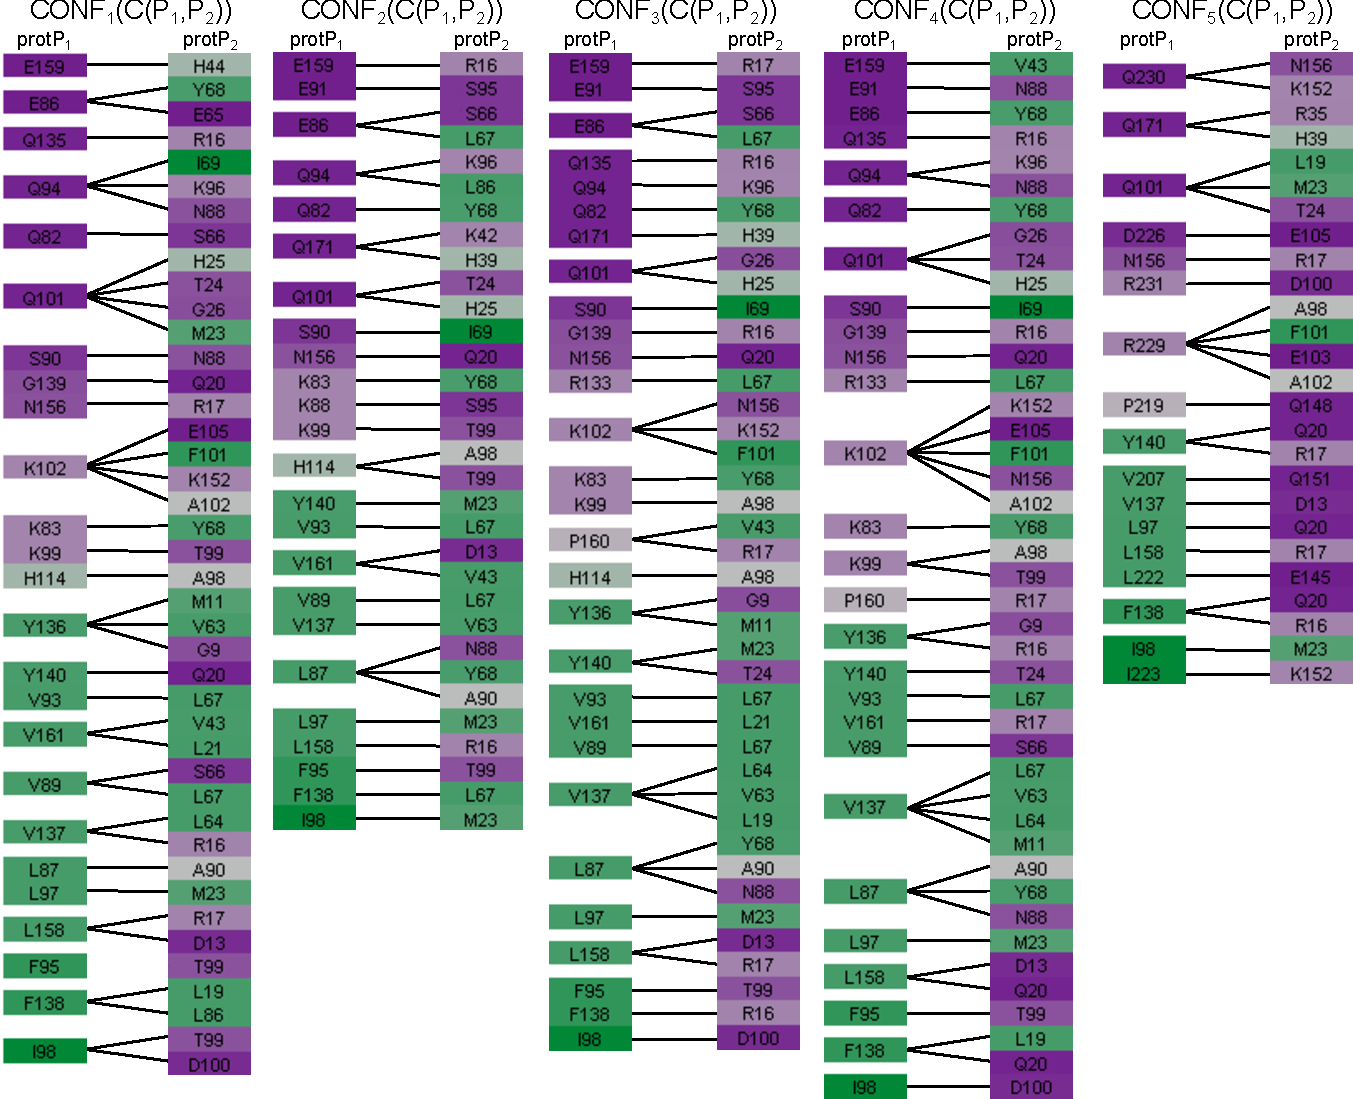
\includegraphics[width=1.0\linewidth]{case3.pdf}
  \caption{Five conformations represented by the juxtapositioned list views, colored and sorted according to hydrophobicity of the amino acids.}
  \label{fig:case3}
\end{figure*}

\textcolor{red}{The end of the case study will be better shaped after the meeting with Honza Palecek on Tuesday.}

\subsection{Case Study 2 -- Blind}
\textcolor{red}{Idea -- to take one representative of each cluster (because in clusters the conformations are similar) and try to find the best solutions. But to find the best ones, I'll need Honza Palecek.}

\section{Conclusion}
In this paper we presented novel visualization methods for exploration and evaluation of biochemical relevance of large sets of conformations detected by existing computational tools.
Our proposed methods were designed to follow the workflow of the domain experts.
We described their design rationale and principles as well as the possible interactions. 
The methods were tested by the domain experts on real datasets of structure maintenance of chromosome complexes and we demonstrated the usability on one of the executed case studies.
The domain experts confirmed that our proposed solution is much more intuitive and user friendly than the previously available methods.
They proved that using our solution their exploration process can lead to a satisfying conclusion about biochemical relevance of individual conformations much faster.

In the future we will extend these methods to complexes consisting of more than than two interacting proteins and build a complete interactive visual analysis tool supporting many tasks performed by the researchers studying protein-protein interactions. 

%% if specified like this the section will be committed in review mode
%\acknowledgments{
%The authors wish to thank A, B, C. This work was supported in part by
%a grant from XYZ. Mobility Rakousko, Mobility Norsko, GAMU}

%\bibliographystyle{abbrv}
\bibliographystyle{abbrv-doi}
%\bibliographystyle{abbrv-doi-narrow}
%\bibliographystyle{abbrv-doi-hyperref}
%\bibliographystyle{abbrv-doi-hyperref-narrow}
%%use following if all content of bibtex file should be shown
%\nocite{*}
\bibliography{template}
\end{document}

